% ============================================================================
% Paper 2 -- integrated from papers/_Computers_in_Biology_and_Medicine__FHIR_driven_Transformation_Pipeline/
% elsarticle-template-num.tex (front matter below transcribed from the elsarticle \title/\author/\affiliation,
% abstract, graphical abstract, highlights and keyword environments; body converted mechanically, see the
% integration report).
% ============================================================================
\section{Towards Real-World Clinical Data Standardization: A Modular FHIR-driven Transformation Pipeline to Enhance Semantic Interoperability in Healthcare}
\label{sec:paper2}

\noindent This section contains the article~\cite{marfoglia_towards_2025}.

\paragraph{Authors.}
Alberto Marfoglia\textsuperscript{a}, Filippo Nardini\textsuperscript{b}, Valerio Antonio Arcobelli\textsuperscript{c}, Serena Moscato\textsuperscript{c}, Sabato Mellone\textsuperscript{c}, Antonella Carbonaro\textsuperscript{a,*}

{\raggedright
\noindent\textsuperscript{a}Dept. of Computer Science and Engineering -- DISI, University of Bologna, Via dell'Universit\`a 50, 47521 Cesena, Italy\\
\textsuperscript{b}Dept. of Electrical, Electronic and Information Engineering ``Guglielmo Marconi'' -- DEI, University of Bologna, Viale del Risorgimento 2, 40136 Bologna, Italy\\
\textsuperscript{c}Dept. of Industrial Engineering -- DIN, University of Bologna, Viale del Risorgimento 2, 40136 Bologna, Italy\\
\textsuperscript{*}Corresponding author. E-mail address: antonella.carbonaro@unibo.it (A. Carbonaro).\\
Computers in Biology and Medicine 187 (2025) 109745. Available online 3 February 2025. 0010-4825/\textcopyright{} 2025 The Authors. Published by Elsevier Ltd. This is an open access article under the CC BY license (\url{http://creativecommons.org/licenses/by/4.0/}).
\par}

\subsection*{Abstract}

\textbf{Background}: Given the exponential increase in clinical data, which accounts for around 30\% of global data volume, effective information management has become crucial to ensuring robust interoperability. This trend is further expedited by implementing consumer-oriented Internet of Things platforms, contributing to the growth of the \$8.3 trillion healthcare industry. These advancements, combined with challenges such as heterogeneous data formats and a lack of incentives, necessitate the development of pragmatic infrastructures and tools that harness contemporary clinical standards like Fast Healthcare Interoperability Resources (FHIR).
\newline
\textbf{Objective}: This study aims to present a modular conversion pipeline employing a templating strategy for translating clinical data into the FHIR model. Emphasis is placed on utilizing a standard mapping specification like FHIR Mapping Language. This ensures essential properties such as platform independence, portability, and code reusability.\newline
\textbf{Methods}: The pipeline was developed incrementally, dividing its core functionalities into five modules: Input, Refinement, Mapping, Validation, and Export. These were subsequently validated by converting a dataset from a prosthetic fitting and rehabilitation center to demonstrate the approach's validity in a real-world data context.\newline
\textbf{Results}: A total of 1962 hospital stay records of 1006 unique patients were converted successfully to 15 distinct types of FHIR resources.
The successful conversion states the pipeline's effectiveness, additionally showcasing its capabilities for enhancing semantic interoperability and facilitating the reuse of real-world data.
\newline
\textbf{Conclusion}: Our approach emerges as a modular data conversion framework that addresses the limitations of existing solutions, making significant contributions to the creation of standardized, interoperable, and high-quality clinical datasets that serve as a foundation for further work.

\subsection*{Graphical abstract}

\begin{center}
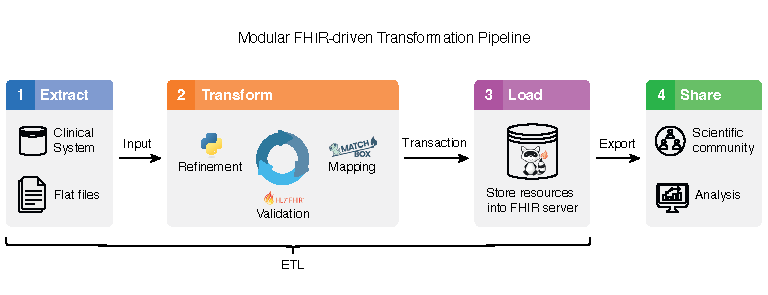
\includegraphics[width=\textwidth]{figures/paper2/grabs.pdf}
\end{center}

\subsection*{Highlights}

\begin{itemize}
\item Development of a modular conversion pipeline utilizing a templating strategy for translating clinical data into the FHIR model.
\item Emphasis on utilizing standard mapping specifications like FHIR Mapping Language for platform independence, portability, and code reusability.
\item Successful validation using a dataset from a center for prosthetic fitting and rehabilitation, confirming semantic preservation.
\item Contribution to creating standardized, interoperable, and high-quality clinical datasets through the enhancement of semantic interoperability and facilitation of real-world data reuse.
\end{itemize}

\paragraph{Keywords:} Health informatics; Standardization; Data conversion; Semantic technology; Software architecture

\subsection{Introduction}
% Please add the following required packages to your document preamble:
% \usepackage{graphicx}
% \begin{table}[t]
% %\begin{tabular}{|l|l|l|}
% \begin{tabular}{|p{0.3\linewidth}|p{0.3\linewidth}|p{0.3\linewidth}|}
% \hline
% \textbf{Problem or Issue} & \textbf{What is Already Known} & \textbf{What this Paper Adds} \\\hline
% Heterogeneous and proprietary clinical data formats hinder interoperability, complicating data reuse and undermining data semantics. & Existing solutions provide conversion pipelines butlack comprehensive, portable, and reusable mapping strategies & Presents a modular conversion pipeline utilizing templating and the FHIR Mapping Language, enhancing interoperability by providing a standardized approach for translating clinical data into the FHIR model. Addresses limitations of existing solutions, facilitating semantic preservation, platform independence, and code reusability.\\\hline
% \end{tabular}%
% \caption{Statement of significance.}
% \label{tab:statement-of-significance}
% \end{table}

% \begin{table}[ht]
% \centering
% \begin{tabular}{|l|p{0.52\linewidth}|}\hline
% \textbf{Problem or Issue} & Heterogeneous and proprietary clinical data formats hinder interoperability, complicating data reuse and undermining data semantics. \\\hline
% \textbf{What is Already Known} & Existing solutions provide conversion pipelines but lack comprehensive, portable, and reusable mapping strategies \\\hline
% \textbf{What this Paper Adds} & Presents a modular conversion pipeline utilizing templating and the FHIR Mapping Language, enhancing interoperability by providing a standardized approach for translating clinical data into the FHIR model. Addresses limitations of existing solutions, facilitating semantic preservation, platform independence, and code reusability.\\\hline
% \end{tabular}%
% \caption{Statement of significance}
% \label{tab:statement-of-significance}
% \end{table}

\begin{table}[ht]
\centering
\resizebox{\textwidth}{!}{ % Adjusts table to fit page width
\begin{tabular}{|l|p{0.9\textwidth}|} % Adjusted column widths for proper wrapping
\hline
\textbf{Problem or Issue} & Heterogeneous and proprietary clinical data formats hinder interoperability, complicating data reuse and undermining data semantics. \\
\hline
\textbf{What is Already Known} & Existing solutions provide conversion pipelines but lack comprehensive, portable, and reusable mapping strategies \\
\hline
\textbf{What this Paper Adds} & Presents a modular conversion pipeline utilizing templating and the FHIR Mapping Language, enhancing interoperability by providing a standardized approach for translating clinical data into the FHIR model. Addresses limitations of existing solutions, facilitating semantic preservation, platform independence, and code reusability. \\
\hline
\end{tabular}
}
\caption{Statement of significance}
\label{tab:paper2_statement-of-significance}
\end{table}

The healthcare landscape is marked by continuous evolution driven by advancements in medical research and technological innovation, resulting in an outstanding growth of clinical data
%CHANGED:
%NEW:
- approximately 30\% of the world’s data volume~\cite{thomason_data_2024}. This growth is further accelerated by the involvement of Big Tech companies in the USD 8.3 trillion healthcare industry. These companies have introduced consumer-focused Internet of Things (IoT) platforms and services, including Amazon Care, Apple’s wearables, and Alphabet’s artificial intelligence (AI)-driven precision medicine initiatives~\cite{thomason_data_2024}. Additionally, emerging technologies such as the IoT and 5G are transforming healthcare, with IoT expected to contribute between USD 0.5–1.8 trillion (14\%) of its total economic value by 2030~\cite{seixas-lopes_musculoskeletal_2024}. The global wearable healthcare market, valued at USD 14.4 billion in 2020, is projected to grow at an annual rate of roughly 18.9\%~\cite{thomason_data_2024}. A significant portion of this growth is driven by home healthcare, which dominated the wearable medical device market in 2021, accounting for 54.5\% of the total revenue~\cite{thomason_data_2024}.

Managing and sharing this information effectively across diverse organizations has emerged as a pivotal challenge on which the progress of the healthcare industry depends~\cite{lehne_why_2019,chatterjee_hl7_2022,kadakia_modernizing_2021}. 
To address this issue, it is essential to develop healthcare systems that are both semantically and structurally cohesive, enabling the seamless exchange of meaningful data. This necessitates the adoption of formal data descriptions, standardized vocabularies, and machine-readable formats~\cite{chatterjee_hl7_2022}. Essentially, interoperability emerges as the linchpin of the digital health revolution~\cite{lehne_why_2019,benson_why_2021}, providing a basis for efficient communication, prospective data curation, and the secondary use of real-world data in medical data science — essential elements for well-informed decision-making. Its economic potential is exemplified by the European Health Data Space (EHDS), which aims to create a unified health data ecosystem. By improving data access in healthcare and facilitating secondary use for research and innovation, the EHDS is projected to save the EU €11 billion over ten years~\cite{qeuropean}.

Despite the mandate in certain regions like the U.S. under the 21st Century Cures Act~\cite{noauthor_21st_2020} requiring the use of the Fast Healthcare Interoperability Resources (FHIR) for health data exchange, many countries lack well-defined regulatory directives and incentives. This has resulted in individual hospitals and software companies adopting custom data formats and interfaces to prioritize short-term gains, thereby hindering interoperability~\cite{benson_why_2021}. To overcome this challenge, standardization is pivotal in achieving data harmonization and improving healthcare information availability, safety, and accuracy~\cite{montazeri2023developing,lehne_why_2019}, as well as integrating heterogeneous data sources. In this context, FHIR, developed by Health Level Seven International (HL7), has emerged as a prominent standard for achieving interoperability in healthcare systems. FHIR conceptualizes healthcare data as modular resources with explicit semantics, offering flexibility and extensibility. This data standard design supports incremental adoption, promoting scalability, cost-effectiveness, and seamless integration into existing healthcare infrastructures~\cite{benson_why_2021}.
Moreover, the FHIR specification can be tailored to suit specific contexts of use through its FHIR profiles mechanism\footnote{https://build.fhir.org/profiling.html}. This feature enables the creation of customized resource definitions by applying constraints and extensions to the base resource. As a result, it promotes standardized implementations that cater to unique requirements effectively.
The recent surge in FHIR adoption can be attributed to its robust framework for exchanging electronic healthcare information and to regulatory measures implemented, particularly in countries like the U.S.~\cite{vorisek_fast_2022}.

% CHANGED:
% NEW:
Recent advancements have underscored FHIR's critical role in ensuring transparency and reproducibility in health data pipelines, particularly for AI-driven applications. Namli et al.~\cite{namli2024scalable} introduced a scalable data preparation pipeline using a declarative language to extract AI-ready datasets from EHR data while ensuring traceability and compliance with emerging regulations like the AI Act. This approach highlights the importance of transparent data transformation processes in creating reproducible AI solutions, addressing challenges such as harmonizing hierarchical FHIR data into AI-compatible formats and handling missing or irregularly sampled clinical data.

% CHANGED:
% NEW:
Emerging applications highlight FHIR's adaptability in tackling healthcare interoperability challenges. For example, platforms integrating Internet of Medical Things (IoMT) devices with 5G network slicing use FHIR to manage data heterogeneity and enable real-time data exchange~\cite{mavrogiorgou_internet_2019}. A scoping review also emphasizes FHIR's expanding role in chronic disease management, including cancer, cardiovascular diseases, and diabetes, within digital health ecosystems~\cite{gazzarata_hl7_2024}. Additionally, FHIR supports modular healthcare platforms that integrate diverse data sources to create standardized Digital Twins (DTs) of patients. These DTs provide semantic-rich foundations for advanced healthcare applications, ensuring data integrity while advancing patient-centric care~\cite{10.3389/fdgth.2023.1322428_carbonaro_connected}.
%
%
% Unfortunately, the lack of well-defined regulatory directives and incentives has resulted in the pervasive adoption of customized data formats and interfaces, primarily motivated by immediate benefits, thereby obstructing interoperability \cite{benson_why_2021}. To overcome this challenge, standardization is pivotal in achieving data harmonization and improving healthcare information availability, safety, and accuracy \cite{montazeri_developing_2023, lehne_why_2019}, as well as integrating heterogeneous data sources. In this context, the Fast Healthcare Interoperability Resources (FHIR), developed by Health Level Seven International (HL7), has emerged as a prominent and widely adopted standard for achieving interoperability in healthcare systems. FHIR conceptualizes healthcare data as modular resources with explicit semantics, offering flexibility and extensibility. This data standard design supports incremental adoption, promoting scalability, cost-effectiveness, and seamless integration into existing healthcare infrastructures \cite{benson_why_2021}. FHIR is the de facto standard for healthcare interoperability, providing a robust framework for representing and exchanging electronic healthcare information.

Nowadays, the focus of most FHIR projects is on developing FHIR-based data infrastructure and pipelines designed to provide standardized data for easy sharing and clinical analysis \cite{duda_hl7_2022}. The key features of these platforms should prioritize incorporating tools facilitating semi-automated data integration and anonymization \cite{gehrmann_what_2023}. Despite progress in this direction \cite{williams2023standardized,xiao_fhir-ontop-omop_2022,kiourtis_structurally_2019,lichtner_representation_2023}, existing solutions face limitations, particularly in terms of portability, code reuse, and maintenance.  

Bennet et al.~\cite{bennett2023mimic} converted the MIMIC-IV database into the FHIR data model to create a real-world FHIR store, an invaluable asset for research. However, the absence of a data sanitization phase and the use of internal mapping logic make the workflow challenging to share. Montazeri et al.~\cite{montazeri2023developing} developed a minimum Data Set customized for Computerized Physician Order Entry (CPOE) in the cardiovascular field, integrated with the Electronic Health Record (EHR) system through the classification and mapping of data elements into FHIR. A notable constraint is the absence of digital tools for the mapping process, necessitating individual and manual verification of each resource. Sinaci et al.~\cite{sinaci2023data} defined and implemented a methodology to enable the FAIR-ification of real-world health data, allowing domain experts to transform existing health data into FHIR via user-friendly GUIs. However, the dependence on an internal mapping language and adopting FHIR profiles, which enforce constraints on resource data fields, impede widespread adoption. Furthermore, Williams et al.~\cite{williams2023standardized} developed an FHIR-based data harmonization pipeline to facilitate an AI-friendly representation of clinical data. Despite its effectiveness, the mapping process implemented in Python and the explicit representation of source database attributes make the mappings strictly dependent on low-level programming details, impeding code reuse. 
% CHANGED:
% NEW:
Ladas et al.~\cite{ladas2022openehr} converted the German Corona Consensus (GECCO) dataset, which describes COVID-19-related patient data, into FHIR to enhance accessibility. Their approach relied on a web-based tool named openEHR-to-FHIR, designed to convert data from the openEHR model into an equivalent GECCO FHIR profile. However, the tool's implementation, which relies on Java classes with regular expressions, limits its reusability for other use cases.
Similarly, Soares et al.~\cite{soares2023omop} developed the OMOP-to-Bulk FHIR tool to process data from an EHR stored in the OMOP Common Data Model (CDM) into FHIR resources. Their workflow involved custom SQL queries to extract data into an intermediate format, which was then transformed into FHIR resources using translation rules. This process was powered by the Whistle Engine, a tool developed by Google that supports FHIR-specific functions and transformations. While effective within the OMOP framework, this solution's dependence on the OMOP CDM as the input data model greatly limits its broader adoption.
Finally, Simon et al.~\cite{simon2024metadata} explored the use of a metadata repository (MDR) to streamline the conversion of data from primary clinical systems into standardized formats. Their methodology involved extracting metadata from hospital forms, defining mappings and transformations in the MDR, and using a REST API to automate the conversion process. Despite its potential, the approach depends heavily on custom scripts, which may hinder generalizability and demand significant effort to adapt to different scenarios.


% CHANGED:
% These approaches reveal challenges arising from manual conversion and validation processes
% NEW:
These approaches, summarized in Table~\ref{tab:paper2_summary}, reveal challenges arising from manual conversion and validation processes and the use of internal mapping languages that hinder the sharing and publishing of mappings. We recognized these shortcomings and defined the essential functionalities necessary for an effective conversion pipeline. These features, detailed in Section \ref{sec:paper2_methods}, guided the development of our solution — a modular framework designed to translate data from various source formats into FHIR seamlessly.

Our approach employs a templating conversion strategy, implemented through the FHIR Mapping Language. This approach enables the definition of mappings in a standardized and declarative manner, empowering users without technical expertise to concentrate only on the data model, and avoiding low-level programming issues. Moreover, our mappings, based on a standard language definition, are language-agnostic and highly portable, facilitating seamless operation on any FHIR server. 

We converted the MOTU dataset to validate our pipeline, a retrospective study evaluating safety against falls and effectiveness for balance and mobility outcomes among different prosthetic knees~\cite{arcobelli_motu_2023}. 

% CHANGED:
% NEW:
The remainder of this manuscript is organized as follows.
Section \ref{sec:paper2_methods} outlines the methodology used in our study, including the pipeline design, architecture, and implementation.
In Section \ref{sec:paper2_results}, we present the results of the data conversion and validation processes.
Section \ref{sec:paper2_discussion} discusses the implications of our findings and potential avenues for future research. It also explores directions for further investigation.
Finally, Section \ref{sec:paper2_conclusion} summarizes the key contributions and provides concluding remarks.


\begin{table}[p]
    \centering
    \resizebox{\textwidth}{!}{ % Adjusts table to fit page width
    \begin{tabular}{|c|p{4cm}|p{4.5cm}|p{4.5cm}|} % Adjust column widths as needed
        \hline
        \textbf{Ref.} & \textbf{Goal} & \textbf{Challenges} & \textbf{Our Approach} \\
        \hline
        \cite{bennett2023mimic} & Convert the MIMIC-IV database into the FHIR data model for a real-world FHIR store & Lack of data sanitization, Internal mapping logic & Elimination of internal mapping logic, standardized and shareable mapping process \\
        \hline
        \cite{montazeri2023developing} & Develop a minimum Data Set for CPOE in the cardiovascular field, integrated with the EHR system & No digital tools for mapping, Individual manual verification required for each resource & Modular, automated mapping system eliminating manual verification \\
        \hline
        \cite{sinaci2023data} & Enable the FAIR-ification of health data using user-friendly GUIs & Dependence on internal mapping language, Enforcing of FHIR Profiles & Language-agnostic, templated approach for defining mappings \\
        \hline
        \cite{williams2023standardized} & Develop an FHIR-based data harmonization pipeline for AI-friendly clinical data representation & Mapping process dependent on Python and explicit source database attributes, limiting code reuse & Portable, reusable framework using standardized mapping language \\
        \hline
        \cite{ladas2022openehr} & Convert COVID-19-related patient data (GECCO) from the openEHR model to FHIR profiles & Implementation based on Java classes and regular expressions, limiting reusability & Reusable, standardized mapping language avoiding reliance on specific implementations \\
        \hline
        \cite{soares2023omop} & Transform EHR data stored in OMOP CDM into FHIR resources & Dependence on the OMOP CDM as the input model, limiting adoption & Flexible framework supporting multiple input models for broader applicability \\
        \hline
        \cite{simon2024metadata} & Automate the conversion of clinical data into standardized formats using an MDR & Reliance on custom scripts, requiring additional effort for generalization and maintenance & Standardized mapping language minimizing reliance on custom scripts \\
        \hline
    \end{tabular}
    }
    \caption{Summary of Related Work: The table outlines the goals and challenges of prior works in the field, highlighting their limitations and how our approach overcomes these gaps to offer novel contributions.}
    \label{tab:paper2_summary}
\end{table}


% \begin{table}[ht]
%     \begin{tabularx}{\textwidth}{|c|l|l|l|}
%         \hline
%          \textbf{Ref.} & \textbf{Goal} & \textbf{Challenges} & \textbf{Our Approach}
%          \\\hline
%          \cite{bennett_mimic-iv_2023} & Convert the MIMIC-IV database into the FHIR data model for a real-world FHIR store & Lack of data sanitization, Internal mapping logic & Elimination of internal mapping logic, standardized and shareable mapping process
%          \\\hline
%          \cite{montazeri_developing_2023} & Develop a minimum Data Set for CPOE in the cardiovascular field, integrated with the EHR system & No digital tools for mapping, Individual manual verification required for each resource & Modular, automated mapping system eliminating manual verification
%          \\\hline
%          \cite{sinaci_data_2023} & Enable the FAIR-ification of health data using user-friendly GUIs & Dependence on internal mapping language, Enforcing of FHIR Profiles & Language-agnostic, templated approach for defining mappings
%          \\\hline
%          \cite{williams_standardized_2023} & Develop an FHIR-based data harmonization pipeline for AI-friendly clinical data representation & Mapping process dependent on Python and explicit source database attributes, limiting code reuse & Portable, reusable framework using standardized mapping language
%          \\\hline
%          \cite{ladas_2022} & Convert COVID-19-related patient data (GECCO) from the openEHR model to FHIR profiles & Implementation based on Java classes and regular expressions, limiting reusability & Reusable, standardized mapping language avoiding reliance on specific implementations 
%          \\\hline
%          \cite{soares_2023} & Transform EHR data stored in OMOP CDM into FHIR resources & Dependence on the OMOP CDM as the input model, limiting adoption & Flexible framework supporting multiple input models for broader applicability
%          \\\hline
%          \cite{simon_2024} & Automate the conversion of clinical data into standardized formats using an MDR & Reliance on custom scripts, requiring additional effort for generalization and maintenance & Standardized mapping language minimizing reliance on custom scripts
%          \\\hline
%     \end{tabularx}
%     \caption{Summary of Related Work and advancements of the proposed solution.}
%     \label{tab:summary}
% \end{table}


% \begin{table}[h]
%     \begin{tabularx}{\textwidth}{|c|X|X|X|}
%         \hline
%          \textbf{Ref.} & \textbf{Focus} & \textbf{Limitations} & \textbf{Our Contribution}
%          \\\hline
%          \cite{bennett_mimic-iv_2023} & Converted MIMIC-IV in FHIR & Absence of data sanitization, Internal mapping logic & Explicit data preprocessing phase, FHIR Mapping Language
%          \\\hline
%          \cite{montazeri_developing_2023} & Developed a dataset for the CPOE in the cardiovascular field & Individual and manual verification of resources & FHIR Server performs validation of produced resources
%          % verifica manuale delle risorse prodotte
%          \\\hline
%          \cite{sinaci_data_2023} & User-friendly GUIs to assist the transformation of health data into FHIR & Internal mapping language, Enforcing of FHIR Profiles & FHIR Mapping Language
%          % internal mapping language, custom profiles
%          \\\hline
%          \cite{williams_standardized_2023} & Data harmonization pipeline to create AI-friendly representation of health data & dependency on technical implementation details, hard to reuse code & FHIR Mapping Language, reusable pipeline
%          % extremely dependent on specific fields + Python + hard to reuse code
%          \\\hline
%     \end{tabularx}
%     \caption{Summary of related works and advancements of the proposed experiment.}
%     \label{tab:summary}
% \end{table}

% The detailed abbreviations and definitions used in the paper are listed in Table \ref{tab:abbreviations}.

% \begin{table}[t]
% \begin{tabular}{|l|l|}
% \hline
% \textbf{Abbreviation} & \textbf{Definition} \\\hline
% ATC & Anatomical Therapeutic Chemical) \\\hline
% CPOE & Physician Order Entry \\\hline
% EHR & Electronic Health Record \\\hline
% ETL & Extract Transform Load \\\hline
% FAIR & Findable, Accessible, Interoperable, and Reusable \\\hline
% FHIR & Fast Healthcare Interoperability Resources \\\hline
% GUI & Graphical User Interface \\\hline
% HAPI FHIR & Java implementation of the HL7 FHIR standard \\\hline
% HL7 & Health Level Seven International \\\hline
% JPA & Java Persistence API \\\hline
% MIMIC & Multi-parameter Intelligent Monitoring for Intensive Care \\\hline
% NLP & Natural Language Processing \\\hline
% RDF & Resource Description Framework \\\hline
% UOM & Units of Measurement \\\hline
% \end{tabular}%
% \caption{List of abbreviations and acronyms used in the paper.}
% \label{tab:abbreviations}
% \end{table}

\subsection{Methods}\label{sec:paper2_methods}
Our work focuses on establishing a conversion pipeline that seamlessly translates data from diverse source formats into modern clinical standards, thereby enhancing healthcare interoperability. This section delineates the development strategy, the architectural framework, the implementation methodologies, and the tools employed in crafting the pipeline. 

\subsubsection{Pipeline design}

\paragraph{Templating Strategy for Declarative Mapping}
Our conversion process relies on a templating strategy that articulates data mappings in a declarative manner. This approach decouples mapping definitions from a specific programming language, promoting flexibility and adaptability across various data models and formats. 

\paragraph{Modular Architecture for Structural Advantages}
The conversion pipeline is structured into modular components, providing several architectural advantages crucial for robustness and scalability: 

\begin{itemize}
    \item \textbf{Maintainability}: The modular design prevents unwanted dependencies between components. This isolation ensures that any requirements alterations impact only the relevant module, minimizing unintended consequences.
    \item \textbf{Incremental Development}: Breaking tasks into distinct components allows for an incremental implementation workflow. This "divide and conquer" approach facilitates a more manageable and systematic development process. 
    \item \textbf{Reusability}: These modular components are designed for reuse across various pipeline implementations. This feature significantly reduces the time needed to address new use cases.
    \item \textbf{Testing and Debugging}: The well-defined responsibilities of each module enable precise control over the software. This granularity simplifies the testing and debugging of smaller, individual components, streamlining the development, and troubleshooting process. 
\end{itemize}

\subsubsection{Pipeline architecture}

The design and development of our pipeline are based on the Extract Transform Load (ETL) framework~\cite{denney_validating_2016}, and its functionalities were organized into sequential modules (Figure~\ref{paper2_1-pipeline-architecture}).  
\begin{enumerate}
    \item \textit{Input}: This module represents the strategy to acquire input data from a specific source, with no restrictions on the input data model and format, as long as a proper API to gather data is provided (e.g., databases, platforms with HTTP API, files, etc.). Additionally, this module addresses data security and regulatory compliance, ensuring that data quality, integrity, and confidentiality are not compromised. 
    \item \textit{Refinement}: This module is designed to preprocess and refine input data. Given the diverse formats and varying quality of the source datasets, this module ensures a uniform output. Moreover, it ensures consistency by eliminating missing data and structuring the information (e.g. using JSON format) to enable seamless conversion operations in subsequent steps. Specifically, the module preserves rows with non-essential null values and removes the ones where missing data are crucial for conveying the meaning of the information.
    \item \textit{Mapping}: This module takes the sanitized source data as input and performs the conversion to the target data model by employing a templating strategy. 
    \item \textit{Validation}: It carries out all the procedures aimed at checking the conformity of output resources with the standard target data model. In case of undesirable outcomes, the module takes immediate action to notify the presence of invalid data. It also initiates any roll-back functions to maintain the integrity of the system's state. 
    \item \textit{Publishing}: The final module executes the necessary logic to store the information in an accessible repository. It also provides essential functionalities, such as querying, exporting, and logging, which enable developers to debug results and design automated tests.
\end{enumerate}

\begin{figure}[ht]
\centerline{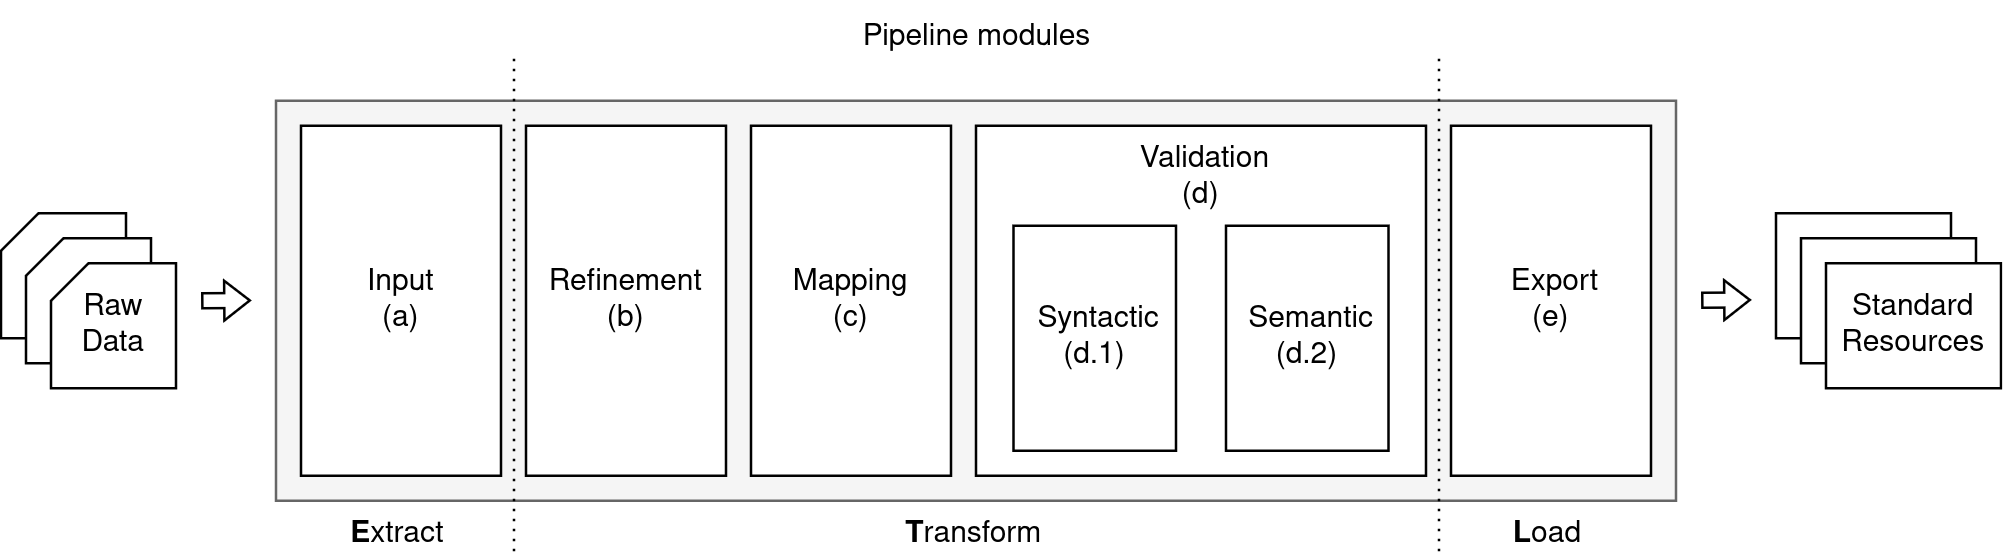
\includegraphics[width=\textwidth]{figures/paper2/1-pipeline-architecture.png}}
\caption{Modules representation of the pipeline architecture, organized according to the Extract, Transform, and Load (ETL) process steps.}
\label{paper2_1-pipeline-architecture}
\end{figure}

\subsubsection{Pipeline implementation}
% CHANGED:
% Our pipeline was methodically constructed in stages, employing data extracted from a relational database and adhering to the HL7 FHIR standard for the output data model. The choice of HL7 FHIR was driven by its flexibility, scalability, and ability to integrate with modern healthcare systems seamlessly, ensuring compatibility and interoperability across diverse data formats and systems in the healthcare domain.
% NEW:
Our pipeline was methodically constructed in stages, employing data extracted from a database and compliant with the HL7 FHIR standard for the output data model. The choice of HL7 FHIR was driven by its flexibility, scalability, and ability to integrate with modern healthcare systems seamlessly, ensuring compatibility and interoperability across diverse data formats and systems in the healthcare domain.

% CHANGED:
% The \textit{Input} (a) and \textit{Refinement} (b) modules (Figure \ref{2-pipeline-implementation}) were implemented using Python scripts supported by data manipulation libraries. These scripts transform the source relational data into sanitized JSON documents for further processing. In our specific case, the developed modules do not include any security checks because the dataset to be converted was already anonymized and verified for quality and integrity at the source.
% NEW: 
The \textit{Input} (a) and \textit{Refinement} (b) modules (Figure \ref{paper2_2-pipeline-implementation}) were implemented using Python scripts supported by data manipulation libraries. These scripts transform the source data into sanitized JSON documents for further processing. In our specific case, the developed modules do not include any security checks because the dataset to be converted was already anonymized and verified for quality and integrity at the source.

The \textit{Mapping} (c) module was developed utilizing Matchbox, a versatile FHIR templating engine characterized by its offline transformation capabilities, allowing standalone microservice deployment, and providing seamless integration as a Java library. Matchbox transforms input JSON object into an FHIR Transaction\footnote{https://build.fhir.org/http.html\#transaction}, a mechanism that empowers clients to send multiple interactions to a server to be processed atomically. This approach adopts the FHIR Bundle Resource as the transport, serving as a container for a collection of FHIR resources. The transactional approach has proved invaluable to performing non-trivial operations, such as storing a collection of related resources, performing conditional creates or updates on existing ones, etc. These features ensure the flexibility of our pipeline to accommodate future evolutions and changing requirements. Matchbox leverages templates defined using the FHIR Mapping Language\footnote{https://build.fhir.org/mapping-language.html} to efficiently transform data from any format to the FHIR data model. Specifically, these templates are parsed into Structure Maps, a detailed set of rules describing the relationships between different data structures, required to enable their automatic conversion. Both the incoming data structures and the resulting FHIR resources are represented by instances of Structure Definition – an FHIR resource that serves as a metamodel for describing schemas. To ensure the integrity of the process, Matchbox conducts syntactic validation (d.1) of the results using the built-in Structure Definitions of the FHIR data model. This step adds a quality control layer, aimed at verifying adherence of produced results with the FHIR specification. 

Upon completion of the pipeline, the HAPI FHIR JPA Server\footnote{https://hapifhir.io/}, an open-source, self-contained solution, was deployed. This server implements storage and retrieval logic without additional coding and exposes a RESTful API. Its primary role involves semantic validation (d.2) of incoming resources concerning the official HL7 Structure Definitions before storing them in the database (e). Lastly, data from the server can be exported in various file formats such as XML, JSON, and FHIR-RDF.

\begin{figure}
\centerline{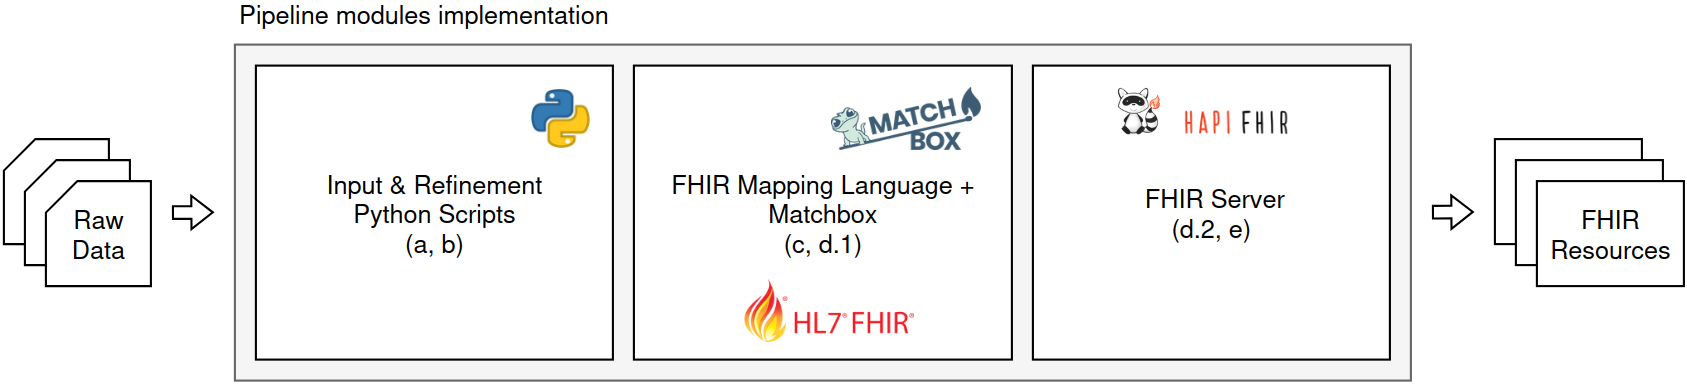
\includegraphics[width=\textwidth]{figures/paper2/2-pipeline-implementation.png}}
\caption{A possible implementation of the pipeline. The identifiers (a, b), (c, d.1), and (d.2, e) refer to the modules of the pipeline architecture shown in Figure \ref{paper2_1-pipeline-architecture}.}
\label{paper2_2-pipeline-implementation}
\end{figure}

\subsubsection{Validation Methodology}
To rigorously assess the accuracy of our pipeline, we focused on converting the MOTU dataset to the FHIR model. MOTU originates from a retrospective observational study conducted at the Italian National Institute for on-the-Job Injuries (INAIL) Prosthesis Center in Budrio, Italy. The study was approved by the Ethics Committee “Area Vasta Emilia Centro” (ref. MOTU 18088, CE AVEC n. 380/2018/OSS/AUSLBO) and complies with the Declaration of Helsinki. It aims to evaluate safety against falls and effectiveness for balance and mobility outcomes among prosthetic knees. The dataset is provided in Comma Separated Values (CSV) format and composed of 1962 hospital stays of 1006 patients with unilateral trans-femoral amputation from January 2011 to May 2020. It includes five tables: Patient, HospitalStay, Fall, DrugHospitalStay, and ProstheticKnee. Patient data feature anonymous IDs, age, and gender, while HospitalStay records admission/discharge dates, amputation details, rehabilitation goals, and assessments on balance, mobility, and daily living activities through questionnaires and functional tests. The Fall table provides information about 146 falls experienced during hospitalizations, detailing prosthesis use and resulting injuries. The DrugHospitalStay table reports information about the medication intake for each hospital stay, listed by trade name and ATC (Anatomical Therapeutic Chemical) code, and counts 3035 instances. The Knee table contains 40 different prosthetic knees, characterized by device details, and manufacturer specifics. To maintain transparency and reproducibility, the input dataset used in this study is publicly available on Zenodo~\cite{arcobelli_motu_2024}. 

% \begin{figure}
% \centerline{\includegraphics[width=\textwidth]{images/4-motu-er.png}}
% \caption{ER schema representing the MOTU dataset.}
% \label{4-motu-er}
% \end{figure}

As a strategy for assessing the completeness and accuracy of the conversion outcomes, we defined five sample queries (Table \ref{tab:paper2_validation-queries}) encompassing a wide range of tables, columns, and data types within the source model. These queries were designed in collaboration with experts from the INAIL, one of Italy's largest prosthetic centers, including a researcher with 30 years of experience and a physical therapist involved in rehabilitating patients with amputations. 
First, we employed the pandas library in Python to execute the queries on the original dataset, ensuring that the logic and criteria set by the domain experts were faithfully replicated. Subsequently, using the SPARQL querying language, we developed corresponding queries replicating the logic of the original ones. This process involved retrieving the FHIR resources in FHIR/RDF format from the HAPI FHIR server's REST API and then uploading them to an Apache Jena Fuseki\footnote{https://jena.apache.org/documentation/fuseki2/} server, an easy to setup open-source SPARQL server that enables simple querying of data through a web interface. The primary goal of such an approach was to compare the resulting number of retrieved instances, aiming for identical outcomes on corresponding queries to confirm the success of the transformation. 

% CHANGED:
% NEW:
To ensure high data quality in the resulting dataset, we adopted the Kahn framework~\cite{kahn_harmonized_2016}, a systematic methodology for data quality assurance. The framework emphasizes three main categories: \textit{Conformance}, which checks the data against syntax and structural constraints; \textit{Completeness}, which ensures that there are no missing values; and \textit{Plausibility}, which assesses the believability and truthfulness of the data values. Each category is further divided into subcategories, providing a detailed structure for quality evaluation (Table~\ref{tab:paper2_kahn-indicators}).

The framework distinguishes between two evaluation contexts: verification, which assesses how well the data aligns with local knowledge and expectations, and validation, which uses external knowledge and benchmarks to evaluate quality. Our study focuses on the verification context, using the precise definitions of data quality of the Kahn framework in all categories to evaluate how effectively our methodology addresses these standards.


\begin{table*}[ht]
\resizebox{\textwidth}{!}{%
\begin{tabular}{|l|l|l|}
\hline
\textbf{Query} & \textbf{MOTU Table(s)} & \textbf{FHIR Resources} \\\hline
Q1: How many patients who came for an initial supply return for a second hospitalization? & HospitalStay & Encounter \\\hline
Q2: How many patients transition from the initial supply of a mechanical knee to a second supply of an electronic knee? & Knee & \begin{tabular}[c]{@{}l@{}}Patient \\ DeviceRequest \\ DeviceDefinition\end{tabular} \\\hline
\begin{tabular}[c]{@{}l@{}}Q3: How many patients use anxiolytics/antidepressants (ATC Code: N06A and N05A) related to the risk of falls?\end{tabular} & Drug & \begin{tabular}[c]{@{}l@{}}Patient \\ Medication \\ MedicationRequest\end{tabular} \\\hline
Q4: Hospital stays from patients over 65 years old? & \begin{tabular}[c]{@{}l@{}}Knee \\ Patient\end{tabular} & \begin{tabular}[c]{@{}l@{}}Patient \\ DeviceRequest\end{tabular} \\\hline
Q5: How many falls per type of prosthesis (AMK, FK, etc.) & \begin{tabular}[c]{@{}l@{}}HospitalStay \\ Fall \\ Knee\end{tabular} & \begin{tabular}[c]{@{}l@{}}DeviceDefinition \\ DeviceRequest \\ Encounter \\ AdverseEvent\\\end{tabular}\\\hline
\end{tabular}%
}
\caption{Demonstration queries used to validate the mapping results. It shows the MOTU tables and the corresponding FHIR resources involved in each query.}
\label{tab:paper2_validation-queries}
\end{table*}

\begin{table*}[ht]
\resizebox{\textwidth}{!}{%
\begin{tabular}{|l|p{5cm}|p{9cm}|} % Adjust column widths
\hline

\multicolumn{1}{|c|}{\textbf{DQA}} & \multicolumn{1}{c|}{\textbf{Description}}                           & \multicolumn{1}{c|}{\textbf{Implementation}}                                                                                                                                                                                                                                                  \\ \hline
Value Conformance                  & Data values conform to allowed formats and values                   & \multirow{3}{=}{Adopting an FHIR Server with strict validation features ensures that data values conform to the correct formats, relational constraints are respected, and required values are always present, thus guaranteeing completeness and data integrity.}                             \\ \cline{1-2}
Relational Conformance             & Data values conform to relational constraints and no duplicate keys &                                                                                                                                                                                                                                                                                               \\ \cline{1-2}
Completeness                       & Absence of data under a predefined threshold                        &                                                                                                                                                                                                                                                                                               \\ \hline
Computational Conformance          & Computed values conform to programming specification                & Computed values, like the number of medications, are not stored, as they can be derived dynamically using FHIRPath queries.                                                                                                                                                                   \\ \hline
Uniqueness Plausibility            & There aren’t two or more resources that identify the same subject   & By adopting FHIR transactions for incremental updates, the risk of creating duplicate resources for the same patient is eliminated.                                                                                                                                                           \\ \hline
Atemporal Plausibility             & Data measures are coherent to a local knowledge                     & \multirow{2}{=}{During the pre-processing phase, Python scripts with custom rules are used to validate input data, ensuring that data adheres to expected properties and is consistent with local knowledge.} \\ \cline{1-2}
Temporal Plausibility              & Data measures are coherent with expected temporal properties        &                                                                                                                \\ \hline
\end{tabular}%
}
\caption{Implementation strategies for the Kahn framework data quality assessments (DQA).}
\label{tab:paper2_kahn-indicators}
\end{table*}

% \begin{table}[ht]
% \begin{tabular}{|l|p{3cm}|p{6cm}|}
% \hline
% \multicolumn{1}{|c|}{\textbf{DQA}} & \multicolumn{1}{c|}{\textbf{Description}}                           & \multicolumn{1}{c|}{\textbf{Implementation}}                                                                                                                                                                                                                                                  \\ \hline
% Value Conformance                  & Data values conform to allowed formats and values                   & \multirow{3}{*}{\parbox{6cm}{Adopting an FHIR Server with strict validation features ensures that data values conform to the correct formats, relational constraints are respected, and required values are always present, thus guaranteeing completeness and data integrity.}}                             \\ \cline{1-2}
% Relational Conformance             & Data values conform to relational constraints and no duplicate keys &                                                                                                                                                                                                                                                                                               \\ \cline{1-2}
% Completeness                       & Absence of data under a predefined threshold                        &                                                                                                                                                                                                                                                                                               \\ \hline
% Computational Conformance          & Computed values conform to programming specification                & Computed values, like the number of medications, are not stored, as they can be derived dynamically using FHIRPath queries.                                                                                                                                                                   \\ \hline
% Uniqueness Plausibility            & There aren’t two or more resources that identify the same subject   & By adopting FHIR transactions for incremental updates, the risk of creating duplicate resources for the same patient is eliminated.                                                                                                                                                           \\ \hline
% Atemporal Plausibility             & Data measures are coherent to a local knowledge                     & \multirow{2}{*}{\parbox{6cm}{During the pre-processing phase, Python scripts with custom rules are used to validate input data, ensuring that data adheres to expected properties and is consistent with local knowledge.}} \\ \cline{1-2}
% Temporal Plausibility              & Data measures are coherent with expected temporal properties        &                                                                                                                                                                                                                                                                                               \\ \hline
% \end{tabular}
% \caption{Implementation strategies for the Kahn framework data quality assessments (DQA).}
% \label{tab:kahn-indicators}
% \end{table}

\subsection{Results}\label{sec:paper2_results}
\begin{figure}
\centerline{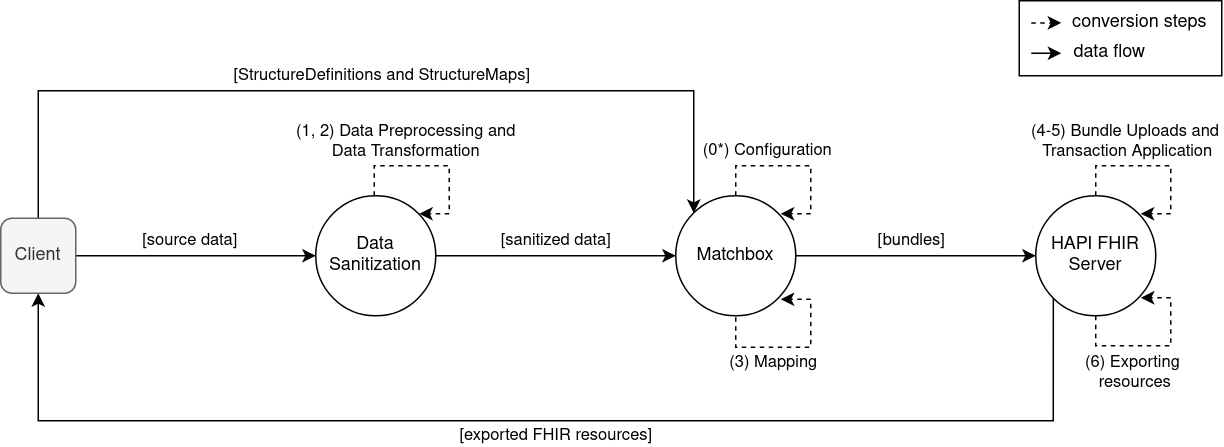
\includegraphics[width=\textwidth]{figures/paper2/3-pipeline-workflow.png}}
\caption{Representation of the role of different services participating in the pipeline. (*) The setup action is performed only once, during the initial configuration on the pipeline.}
\label{paper2_3-pipeline-worflow}
\end{figure}

The implemented pipeline successfully converted the MOTU dataset into FHIR-compliant resources~\cite{arcobelli2024fhir}. The transformation process, leveraging the previously described modules, encompassed the following key steps (Figure \ref{paper2_3-pipeline-worflow}): 

\begin{itemize}
    \item \textbf{Configuration Setup (Step 0)}: Upon deployment, the pipeline was configured by uploading Structure Definitions and Structure Maps obtained in collaboration with MOTU dataset experts~\cite{arcobelli_motu_2023}. 
    \item \textbf{Data Preprocessing (Step 1)}: Raw data from the MOTU dataset~\cite{arcobelli_motu_2024} underwent a thorough preprocessing step by using data sanitization services. This step ensured data quality, consistency, and compatibility with subsequent pipeline stages. 
    \item \textbf{Data Transformation (Step 2)}: The CSV data was transformed into JSON objects to streamline processing by Matchbox. This step included renaming, typing, and filtering source data fields. 
    \item \textbf{Mapping (Step 3)}: Matchbox transformed each JSON object into an FHIR Transaction. Moreover, Matchbox performed a syntactic validation to ensure the correctness of input and output data schemas. 
    \item \textbf{Bundles Upload (Step 4)}: Generated Bundles were dispatched individually to the HAPI FHIR server to validate and store the enclosed resources. Placeholder IDs, temporary and randomly generated UUIDs, were used to link resources within the Bundle, facilitating the determination of corresponding concepts and preventing duplications. 
    \item \textbf{Transaction Application (Step 5)}: Upon arrival at the HAPI FHIR server, Bundles underwent a processing step with reference integrity checks, resolution of temporary UUIDs, and assessment of resource conformity to FHIR profiles using the server's integrated FHIR Instance Validator module\footnote{https://hapifhir.io/hapi-fhir/docs/validation/instance\_validator.html}. This will use terminology services to validate codes, and StructureDefinitions to validate semantics. Successful transactions modified the state of the server, enabling incremental updates to the same resource from subsequent Bundles. On the other hand, failed transactions triggered a complete rollback to the previous state, ensuring successful storage only upon error-free processing. 
    \item \textbf{Exporting Resources (Step 6)}: All stored resources within the HAPI FHIR server resulting from the conversion process were exported in NDJSON format using the server's built-in FHIR Bulk Data Access protocol. This operation organized FHIR resources by their type and segmented them into files. The resulting FHIR resources dataset can be accessed on Zenodo~\cite{arcobelli_fhired_2024}.
\end{itemize}

A concrete example of data workflow conversion is illustrated in Figure \ref{paper2_5-data-conversion-workflow}. In Step 1, the initial phase entailed data sanitization, involving the removal of unused columns, and the conversion of dates into the ISO 8601 format. Afterward, in Step 2, the data is transformed into JSON format, enabling its utilization through Matchbox (Figure \ref{paper2_5-data-conversion-workflow}.b).
Step 3 encompassed the mapping of the source data onto a Bundle comprising FHIR-compliant resources, each identified by temporary UUIDs, thereby enabling seamless cross-referencing (Figure \ref{paper2_5-data-conversion-workflow}.c). Notably, the semantic richness of FHIR resources was enhanced by the integrating formal CodeSystems. Subsequently, the Bundle was transmitted to the HAPI FHIR server to execute the necessary transaction (Step 4). Finally, in Step 5, the resultant FHIR resources were individually stored in the HAPI FHIR server, and their temporary UUIDs were substituted with universal ones to enable their integration with the existing knowledge (Figure \ref{paper2_5-data-conversion-workflow}.d).

% CHANGED:
% NEW:
The experiment was conducted on a system with an Intel Core i9-14900KF processor (32 cores) and 128 GB of RAM, running Ubuntu 24.04.1 LTS. The pipeline converted the entire MOTU dataset in 8 minutes and 52.467 seconds.

\begin{figure}
\centerline{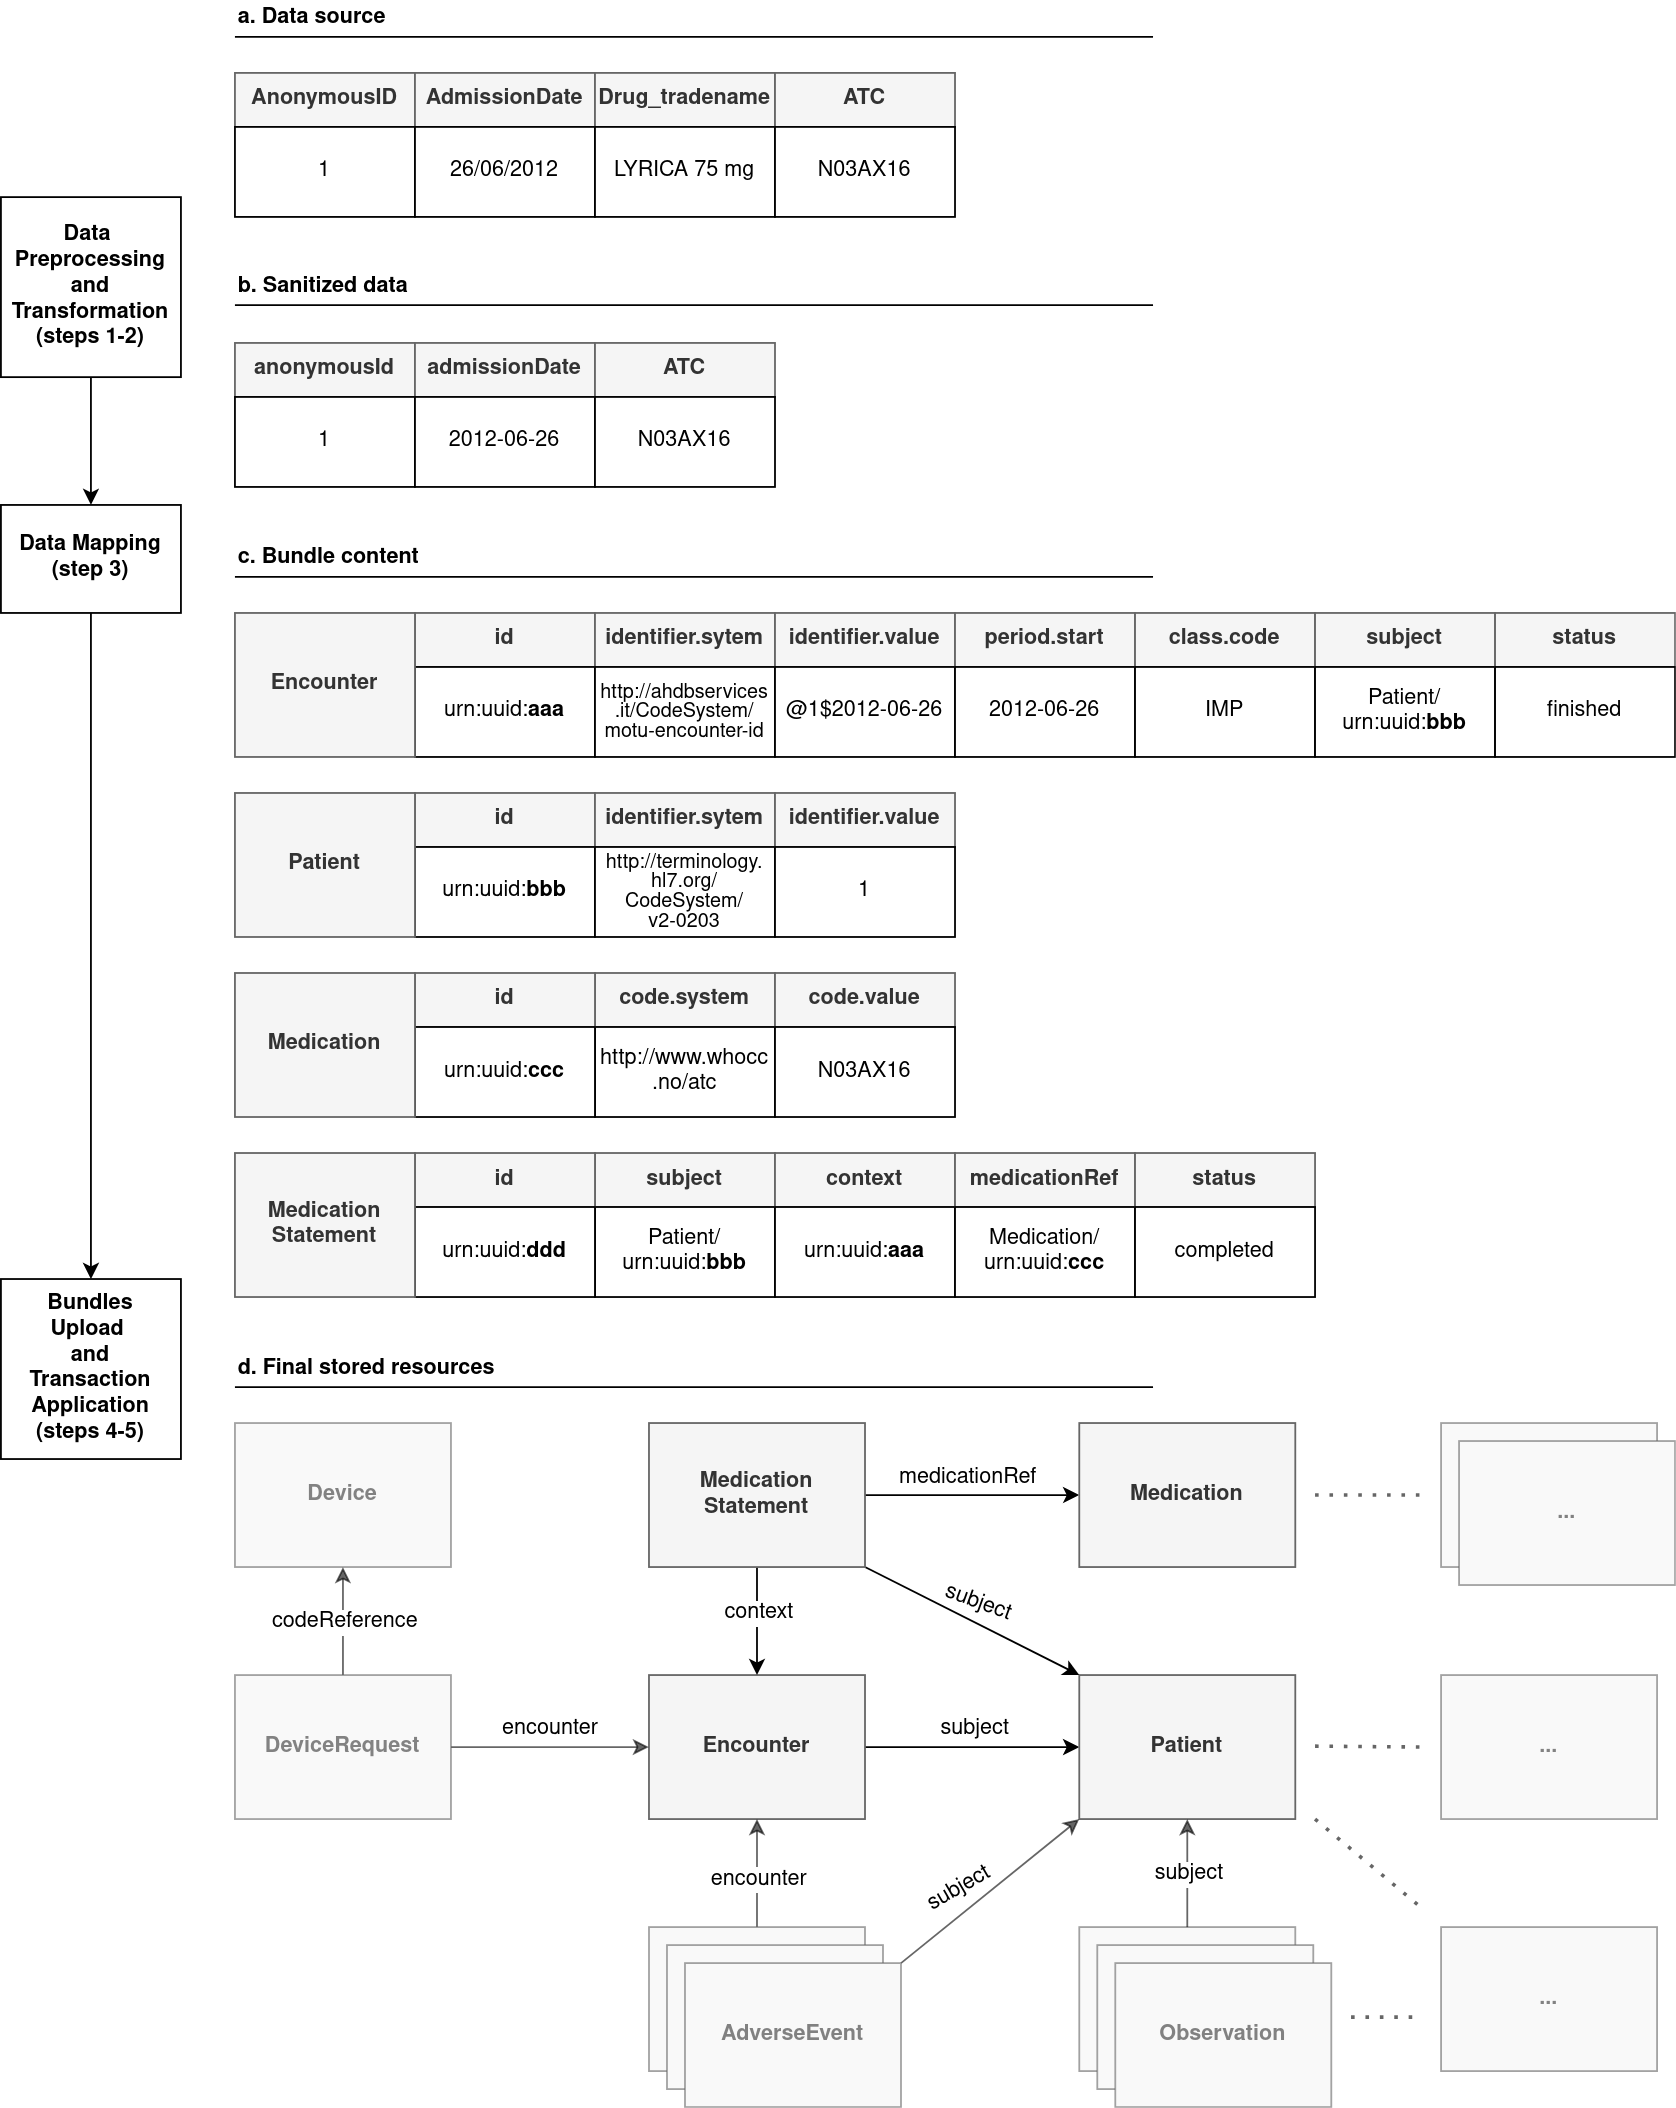
\includegraphics[width=\textwidth]{figures/paper2/4-data-conversion-workflow.png}}
%\caption{Simplified representation of a real-world example of data conversion workflow. It highlights all the crucial transformation steps from the source dataset (MOTU DrugHospitalStay table) to the FHIR domain. The resources produced in step 3 are implicitly organized inside a Bundle. Finally, in steps 4-5 the converted resources will be integrated with the prior knowledge.}
\caption{Diagram showing data conversion workflow from MOTU DrugHospitalStay table to FHIR domain, bundling resources in step 3, and integrating them with prior knowledge in steps 4-5."}
\label{paper2_5-data-conversion-workflow}
\end{figure}

\subsubsection{Implemented Mappings}

% \begin{table*}[t]
% \resizebox{\textwidth}{!}{%
% \begin{tabular}{|l|l|c|l|}
% \hline
% \textbf{MOTU} & \textbf{FHIR} & \textbf{Total resources} & \textbf{Usage} \\
% \hline
%  & Encounter & 1960 & Models the Information about the hospitalization of a patient \\
% \hline{1-3}
%  & QuestionnaireResponse & 23520 & Models the responses to standard questionnaires (Barthel, Morse, etc.) \\
%  & Account & 1960 &  \\
%  & Coverage & 1960 & \multirow{-2}{*}{Outline the entity in charge of payment} \\
%  & Observation & 11697 & Describes the measurements and the analysis results performed during the hospitalization \\
%  & Procedure & 1960 & Defines an intervention of amputation (body part, cause, date) \\
%  & Condition & 181 & Models any patient’s disorders, such as diabetes. \\
%  & DeviceRequest & 1835 & Model a request for knee prosthesis \\
%  & Careplan & 1960 &  \\
% \multirow{-10}{*}{HospitalStay} & Goal & 1960 & \multirow{-2}{*}{Describe the rehabilitation and the achieved goals} \\
% Knee & DeviceDefinition & 40 & Defines the properties of a certain model of knee prosthesis \\
%  & Medication & 370 &  \\
% \multirow{-2}{*}{Drug} & MedicationStatement & 3032 & \multirow{-2}{*}{Describe a drug and its prescriptions} \\
%  & AdverseEvent & 147 & Models a fall event associated with the hospitalization. \\
% \multirow{-2}{*}{Fall} & DocumentReference & 147 & Captures all the textual notes linked to the fall event \\
% Patient & Patient & 1005 & Models the patient's details \\\hline
% \end{tabular}%
% }
% \caption{Shows high-level mappings between MOTU tables and FHIR resources. These mappings establish a central reference point - Encounter, DeviceDefinition, Medication, AdverseEvent, and Patient - since it is referenced by all other resources derived from the same MOTU table's mapping process. }
% \label{tab:motu-references}
% \end{table*}

\begin{table*}[ht]
\resizebox{\textwidth}{!}{%
\begin{tabular}{|l|l|c|l|}
\hline
\textbf{MOTU} & \multicolumn{1}{c|}{\textbf{FHIR}} & \multicolumn{1}{c|}{\textbf{Total resources}} & \multicolumn{1}{c|}{\textbf{Usage}} \\ \hline
\multirow{10}{*}{HospitalStay} & Encounter & 1962 & Models the Information about the hospitalization of a patient \\ \cline{2-4} 
 & QuestionnaireResponse & 23544 & Models the responses to standard questionnaires (Barthel, Morse, etc.) \\ \cline{2-4} 
 & Account & 1962 & \multirow{2}{*}{Outline the entity in charge of payment} \\ \cline{2-3}
 & Coverage & 1962 &  \\ \cline{2-4} 
 & Observation & 11709 & Describes the measurements and the analysis results performed during the hospitalization \\ \cline{2-4} 
 & Procedure & 1962 & Defines an intervention of amputation (body part, cause, date) \\ \cline{2-4} 
 & Condition & 181 & Models any patient’s disorders, such as diabetes. \\ \cline{2-4} 
 & DeviceRequest & 1835 & Model a request for knee prosthesis \\ \cline{2-4} 
 & Careplan & 1962 & \multirow{2}{*}{Describe the rehabilitation and the achieved goals} \\ \cline{2-3}
 & Goal & 1962 &  \\ \hline
Knee & DeviceDefinition & 40 & Defines the properties of a certain model of knee prosthesis \\ \hline
\multirow{2}{*}{Drug} & Medication & 370 & \multirow{2}{*}{Describe a drug and its prescriptions} \\ \cline{2-3}
 & MedicationStatement & 3032 &  \\ \hline
Fall & AdverseEvent & 146 & Models a fall event associated with the hospitalization. \\ \hline
Patient & Patient & 1006 & Models the patient’s details \\ \hline
\end{tabular}%
}
\caption{Shows high-level mappings between MOTU tables and FHIR resources. These mappings establish a central reference point - Encounter, DeviceDefinition, Medication, AdverseEvent, and Patient - since it is referenced by all other resources derived from the same MOTU table’s mapping process.}
\label{tab:paper2_motu-references}
\end{table*}

% CHANGED: 
% The pipeline conversion process involves 157 fields of MOTU tables, covered by 15 distinct types of FHIR resources (Table \ref{tab:motu-references}).
% A correspondence with FHIR variables was found for 155 fields, representing 98.7\% of the dataset, of which 143 (91.1\%) were mapped to FHIR resources fields, and 12 identified as computable values through FHIRPath expressions.
% NEW:
The pipeline conversion process involves 157 fields from the MOTU tables, mapped to 15 distinct types of FHIR resources (Table \ref{tab:paper2_motu-references}). A correspondence to FHIR variables was established for 155 fields, covering 98.7\% of the dataset~\cite{arcobelli2024fhir}. Of these, 143 fields (91.1\%) were directly mapped to FHIR resource fields, while the remaining 12 (1.3\%) fields were recognized as computable values through FHIRPath expressions.
Several external ontologies, such as LOINC\footnote{https://loinc.org/}, SNOMED-CT\footnote{https://www.snomed.org/}, and Units of Measurement (UOM)\footnote{https://units-of-measurement.org/} ontology were adopted, to provide the results with a precise, consistent, and machine-readable representation of clinical concepts. As the information from the source dataset is specific, a corresponding concept from standard vocabularies was sometimes missing. Different Code Systems were created to overcome this lack of coverage. Moreover, before initiating the pipeline, shared concepts between all the records, such as Questionnaires, and Organizations were manually created and uploaded to the FHIR server. 

% CHANGED: 
% During our analysis of the dataset, we found redundant information in the source tables, such as the count of prescribed drugs during hospitalization. To avoid data duplication, inconsistencies, and potential errors, we decided not to include this information in the FHIR data model. We can still derive such pieces of information by using ad-hoc Search Parameters that incorporate FHIRPath expressions, which are accessible through the FHIR RESTful API.
% NEW:
% TODO: Controlla 157 variabili da dove vengono. Nel paragrafo sopra si parla di 75 fields.
% Of the initial 157 variables in the CSV dataset, we successfully established a correspondence with FHIR for 155 variables, representing 98.7\% of the dataset. We mapped 143 variables (91.1\%) to FHIR resources and identified 12 variables (1.3\%) that can be derived from FHIRPath expressions~\cite{moscato2024fhir}.

\subsubsection{Validation}
The validation process for resources derived from the MOTU dataset involved utilizing FHIRPath queries executed on the HAPI FHIR Server, and Python scripts for analyzing the original dataset. Initially, the validation encompassed counting the "root" resources, signifying overarching concepts uniquely identified by a primary key within the MOTU tables. This count was subsequently compared to the total number of rows within the tables, as outlined in Table \ref{tab:paper2_motu-convertion-results}. The consistent alignment of query counts across all assessments confirmed the accurate transformation of the core concepts of the MOTU domain. 
% CHANGED:
% In the validation test, utilizing queries provided by domain experts (Table \ref{tab:validation-queries}), we found consistent outcomes across both groups of queries (Table \ref{tab:motu-convertion-comparison}).
% NEW: attaccato paragrafo e cambiato "In the validation test" -> "Subsequently"
Subsequently, utilizing queries provided by domain experts (Table \ref{tab:paper2_validation-queries}), we found consistent outcomes across both groups of queries (Table \ref{tab:paper2_motu-convertion-comparison}).

% CHANGED:
% NEW:
% Identifying Relevant FHIR Elements for Data Quality Assessment in the German Core Data Set
% The OMOP common data model in Australian primary care data: Building a quality research ready harmonised dataset
% A Harmonized Data Quality Assessment Terminology and Framework for the Secondary Use of Electronic Health Record Data
% Development and initial validation of a data quality evaluation tool in obstetrics real-world data through HL7-FHIR interoperable Bayesian networks and expert rules
% Forse lo metterei in methodologies se diciamo che non sono verifiche, ma piu garanzie date dalla metodologia di lavoro


\begin{table}[ht]
\begin{tabular}{|l|l|c|c|}
\hline
\textbf{MOTU Table} & \textbf{FHIR Resource} & \textbf{No. MOTU} & \textbf{No. FHIR} \\ \hline
HospitalStay & Encounter & 1962 & 1962 \\ \hline
Knee & DeviceDefinition & 40 & 40 \\ \hline
Drug & MedicationStatement & 3035 & 3032* \\ \hline
Fall & AdverseEvent & 146 & 146 \\ \hline
Patient & Patient & 1006 & 1006 \\ \hline
\end{tabular}%
\caption{Comparison of distinct item counts in the original dataset and the corresponding FHIR “root” resources derived from mapping. Results are aligned, except for three MedicationStatement entries (*) excluded due to lacking ATC codes.}
\label{tab:paper2_motu-convertion-results}
\end{table}

% Please add the following required packages to your document preamble:
% \usepackage{graphicx}
% \usepackage[table,xcdraw]{xcolor}
% Beamer presentation requires \usepackage{colortbl} instead of \usepackage[table,xcdraw]{xcolor}
\begin{table}[ht]
\resizebox{\textwidth}{!}{%
\begin{tabular}{|l|c|c|}
\hline
\textbf{Query} & \textbf{Python count} & \textbf{SPARQL count} \\ \hline
Q1: How many patients who came for an initial supply return for a second hospitalization? & 85 & 85 \\ \hline
Q2: How many patients transition from the initial supply of a mechanical knee to a second supply of an electronic knee? & 34 & 34 \\ \hline
Q3: How many patients use anxiolytics/antidepressants (ATC Code: N06A and N05A) related to the risk of falls? & 67 & 67 \\ \hline
Q4:  Hospital stays from patients over 65 years old & 674 & 674 \\ \hline
Q5: How many falls per type of prosthesis (AMK, FK, etc.) & \begin{tabular}[c]{@{}l@{}}AMK - 11  \\ FK - 79  \\ LK - 26  \\ MPK - 28\end{tabular} & \begin{tabular}[c]{@{}l@{}}AMK - 11  \\ FK - 79  \\ LK - 26  \\ MPK - 28\end{tabular} \\ \hline
\end{tabular}%
}
\caption{Summary of results from demonstration queries. The total count for query Q5 is 144, reflecting the exclusion of two rows from the HospitalStay table due to the absence of any reference to the prosthesis model, leading to their omission in the inner join operation.}
\label{tab:paper2_motu-convertion-comparison}
\end{table}

% \begin{table}[]
% \resizebox{\textwidth}{!}{%
% \begin{tabular}{|l|l|l|}
% \hline
% \multicolumn{1}{|c|}{\textbf{DQA}} & \multicolumn{1}{c|}{\textbf{Description}}                           & \multicolumn{1}{c|}{\textbf{Implementation}}                                                                                                                                                                                                                                                  \\ \hline
% Value Conformance                  & Data values conform to allowed formats and values                   & \multirow{3}{*}{Adopting a FHIR Server with strict validation features ensures that data values conform to the correct formats, relational constraints are respected, and required values are always present, thus guaranteeing completeness and data integrity.}                             \\ \cline{1-2}
% Relational Conformance             & Data values conform to relational constraints and no duplicate keys &                                                                                                                                                                                                                                                                                               \\ \cline{1-2}
% Completeness                       & Absence of data under a predefined threshold                        &                                                                                                                                                                                                                                                                                               \\ \hline
% Computational Conformance          & Computed values conform to programming specification                & Computed values, like the number of medications, are not stored, as they can be derived dynamically using FHIRPath queries.                                                                                                                                                                   \\ \hline
% Uniqueness Plausibility            & There aren’t two or more resources that identify the same subject   & By adopting FHIR transactions for incremental updates, the risk of creating duplicate resources for the same patient is eliminated.                                                                                                                                                           \\ \hline
% Atemporal Plausibility             & Data measures are coherent to a local knowledge                     & \multirow{2}{*}{During the pre-processing phase, Python scripts with custom rules are used to validate input data, ensuring that temporal data adheres to expected time properties and that atemporal data is consistent with local knowledge and does not depend on time-sensitive factors.} \\ \cline{1-2}
% Temporal Plausibility              & Data measures are coherent with expected temporal properties        &                                                                                                                                                                                                                                                                                               \\ \hline
% \end{tabular}
% }%
% \caption{Implementation strategies for the Kahn framework data quality assessments (DQA).}
% \label{tab:kahn-indicators}
% \end{table}

\subsection{Discussion}\label{sec:paper2_discussion}
We successfully designed and implemented a modular FHIR-based conversion pipeline capable of extracting, preprocessing, and standardizing real-world health data.
Validation, performed on the MOTU dataset, ensures that the transformed data maintains accuracy and meaning. Consistent counts validated the preservation of core concepts, while clinician-driven queries affirmed the retention of semantic integrity and relational coherence. This comprehensive validation reinforces the trustworthiness of the transformed FHIR resources in capturing the essence of the MOTU domain. The resulting FHIR-conformant resources enhance interoperability, support high-throughput computation~\cite{hong_developing_2019}, and improve accessibility and readability for both humans and machines. This achievement is reinforced by the integration of standard ontologies, contributing to enriched semantic content and reduced ambiguities. Furthermore, the generated resources are efficiently findable through the RESTful Search API – a critical component for realizing a scalable platform capable of handling extensive volumes of information. Our harmonization process yields output with a greater volume than the input, attributable to the inclusion of metadata, mandatory fields, and references to external ontologies or concepts within FHIR resources. Managing this expanded knowledge corpus necessitates the deployment of automated software infrastructures, as emphasized in prior research~\cite{gehrmann_what_2023}. 

The implemented pipeline provides a versatile and scalable framework to support the FHIR modeling of custom data, including modules aimed at streamlining semi-automated data integration. The validation module removes the need for manual evaluation, cutting down time and reducing errors. This is pivotal for achieving semantic and structural interoperability in health information, identified as a significant research challenge in recent years~\cite{chatterjee_hl7_2022,kadakia_modernizing_2021}. As demonstrated with the MOTU dataset, this framework could play a crucial role in addressing a key aspect of digital health research — facilitating the comprehensive and meaningful reuse of real-world data. This capability is vital for supporting analyses in the field of Medical Data Science~\cite{gehrmann_what_2023}. 

In the realm of health informatics, the showcased pipeline exhibits several remarkable strengths that distinguish it from existing approaches. Primarily, its modular design ensures scalability and adaptability for a broad range of clinical studies and data sources, providing a versatile solution applicable across various scenarios. Notably, the adoption of Bundle transactions significantly enhances efficiency, enabling the processing of large datasets at speeds up to 50 times\footnote{https://smilecdr.com/docs/fhir\_standard/transactions.html} faster than individual operations. Furthermore, utilizing the RESTful interface provided by the FHIR server allows for parallel processing of bundles, further enhancing overall performance. 

An essential feature of the framework is its automated validation mechanism, systematically ensuring the adherence of each FHIR resource to the FHIR model. This procedure, supported by Structure Definitions and Structure Maps, distinguishes our study from others that rely on manual validation processes~\cite{montazeri2023developing}. Additionally, the adoption of a templating conversion strategy introduces a language-agnostic approach. This empowers users to concentrate exclusively on the mapping activity, irrespective of their technical proficiency. This eliminates the necessity for alterations to the framework code, allowing users to navigate the conversion process without requiring expertise in specific programming languages. 

Unlike similar solutions such as the .NET-based FHIR Converter\footnote{https://github.com/microsoft/FHIR-Converter}, limited to handling specific source data types (HL7 version 2 and CDA), our pipeline boasts versatility by accommodating any input format. In addition, adopting the FHIR Mapping Language not only formalizes the conversion process but also makes it externally accessible and publishable. This distinctive feature promotes transparency in our mappings, a quality often lacking in comparable studies~\cite{sinaci2023data,williams2023standardized}. 

The primary limitation of our research lies in its validation, which was exclusively conducted using the MOTU dataset. To enhance the robustness of our solution, our objective is to broaden the validation scope to encompass a wider range of datasets. This step is crucial for unveiling potential challenges and obstacles while assessing the practical adaptability of our pipeline architecture across diverse scenarios. For instance, it should be noted that, for the MOTU dataset, creating FHIR profiles was not necessary to handle explicit constraints given by domain-specific rules or requirements. On the contrary, other datasets may require the definition of FHIR profiles. As an example, the US Core FHIR profile\footnote{http://hl7.org/fhir/us/core/} provides its definitions for many FHIR resources, such as the Patient resource, which includes mandatory fields such as name and additional fields such as date of death, not natively mandatory in the basic Patient resource. The inclusion of FHIR profiles creation must be seamlessly integrated into our pipeline to map the structure and characteristics of the source information, avoiding any loss of context or meaning.

Other limitations arise from the current manual procedures for implementing ad-hoc input/refinement scripts and defining mappings. These tasks, inherently domain-specific, require substantial time and effort investment. A promising path for improvements involves exploring the implementation or integration of Natural Language Processing (NLP), as exemplified in Google's Healthcare Natural Language API\footnote{https://cloud.google.com/healthcare-api/docs/how-tos/nlp?hl=it }. NLP tools can be used to automatically extract structured data from unstructured clinical documents~\cite{hong_developing_2019} and to assist in creating mappings by suggesting the most suitable FHIR resources and external ontology codes to model specific concepts. In this regard, we are developing an automatic mapping tool that uses NLP to convert textual descriptions of variables into FHIR resources. By fine-tuning the model with FHIR documentation, the tool will act as a decision support system, suggesting outcomes that operators can review and approve. To enhance usability for non-technical users and streamline the process, these tools should feature a graphical user interface, ultimately saving time and simplifying the mapping workflow.

Finally, to enhance the efficiency of the overall post-hoc validation step, we are working on automation to streamline procedures. This involves integrating automated functionalities into a new pipeline module, aligned with DevOps principles. This module will orchestrate a series of tasks triggered by changes in mapping logic or source dataset. For instance, the generated FHIR resources will be converted directly into RDF format and integrated into a pre-deployed knowledge graph repository, like Apache Jena Fuseki. Afterward, predefined queries in configuration files will be analyzed against both input and output providing a comprehensive summary of results.
Automating these tasks facilitates seamless coverage and ensures consistent application of semantic integrity tests. Importantly, this approach decouples the technical implementation from the semantics of the queries outlined by non-technical users, significantly enhancing the acceptance process and pipeline usability.

\subsection{Conclusion}\label{sec:paper2_conclusion}
This paper presents an FHIR-based conversion pipeline designed to enhance the interoperability of real-world health data. The transition to a modern clinical standard, such as HL7 FHIR, represents a pivotal step towards unlocking latent value within heterogeneous data silos. Our solution, characterized by its modular architecture and templating mapping strategy based on the FHIR Mapping Language, offers a flexible and scalable approach to implementation, effectively addressing the complexities inherent in health data management. Furthermore, the employed templating approach ensures the formalization of mappings, providing an implementation-independent solution suitable for external publication. 
% CHANGED:
% NEW: attacca paragrafo
The effectiveness of our proposed solution underwent rigorous validation against the MOTU dataset. Through well-conceived queries on both the source dataset and the output generated by the pipeline, we demonstrated the pipeline's ability to seamlessly transform the MOTU dataset into FHIR without compromising accuracy or completeness.  

% CHANGED:
% Looking forward, future works involve the comprehensive validation of the pipeline across diverse datasets, considering variations in quality, format, and volume. As previously discussed, our emphasis lies in developing tools to streamline the mapping definition process, identified as a crucial bottleneck in the conversion workflow. By addressing these aspects, we aim to solidify the applicability and scalability of our FHIR-based conversion pipeline in real-world settings, effectively addressing prevailing challenges in health data interoperability. 
% NEW:
Building on these achievements, future efforts will prioritize expanding validation across diverse datasets, encompassing variations in structure, quality, and domain-specific requirements. Incorporating FHIR profile creation, where needed, will ensure that domain constraints are met without losing context or meaning. To address the manual bottlenecks in mapping and refinement, we plan to integrate advanced automation techniques, including natural language processing, to support variable extraction and mapping processes. Developing intuitive graphical interfaces for these tools will empower non-technical users, fostering broader adoption and usability.

Additionally, enhancing the automation of post-hoc validation through DevOps-aligned modules will streamline workflows, ensuring consistency and semantic coherence across all outputs. The incorporation of automated RDF conversion and semantic integrity tests within knowledge graphs will further reinforce the reliability of the pipeline while decoupling technical complexities from user interactions.

By addressing these aspects, we aim to solidify the applicability and scalability of our FHIR-based conversion pipeline in real-world settings, effectively addressing prevailing challenges in health data interoperability.

\subsection*{Acknowledgment}
This research was co-funded by the Complementary National Plan PNC-I.1 “Research initiatives for innovative technologies and pathways in the health and welfare sector” D.D. 931 of 06/06/2022, DARE - DigitAl lifelong pRevEntion initiative, code PNC0000002, CUP: 
(B53C22006450001) and by the Italian National Institute for Insurance against Accidents at Work (INAIL) within the MOTU++ project (PR19-PAI-P2). Authors express their gratitude to the AlmaHealthDB Team.

\subsection*{Code availability}
The MOTU-to-FHIR Mapping Pipeline code is available on GitLab at \url{https://gitlab.com/almahealthdb/ahdb-mapping-service/}. This repository includes all the necessary scripts, configuration files, and guidelines for converting the MOTU CSV dataset into a FHIRed dataset according to the HL7 FHIR standard (R4 version). It also offers a Docker Compose file configuring Matchbox and the HAPI FHIR Server, enabling automated pipeline deployment. For detailed instructions on running the pipeline, please refer to the README.md file in the repository.

% layout: keep this paper's floats within its section
\FloatBarrier
